% Created by tikzDevice version 0.10.1 on 2016-08-15 14:58:40
% !TEX encoding = UTF-8 Unicode
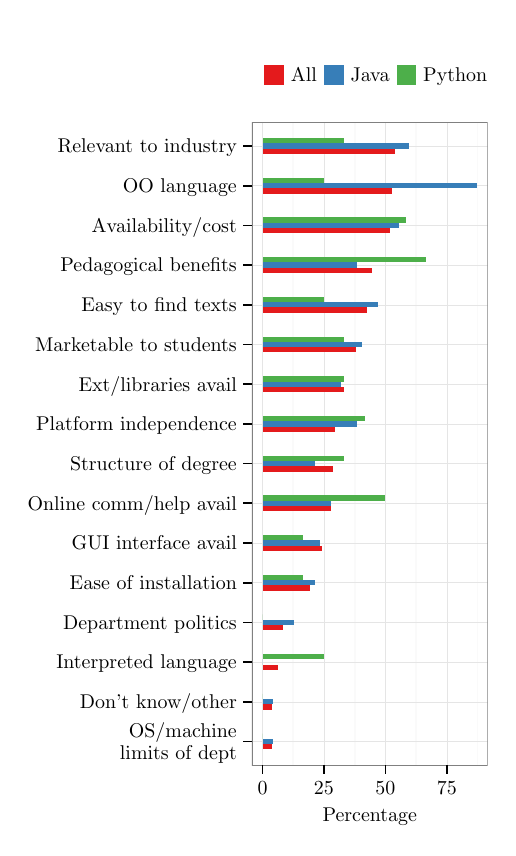
\begin{tikzpicture}[x=1pt,y=1pt]
\definecolor{fillColor}{RGB}{255,255,255}
\path[use as bounding box,fill=fillColor,fill opacity=0.00] (0,0) rectangle (166.22,289.08);
\begin{scope}
\path[clip] (  0.00,  0.00) rectangle (166.22,289.08);
\definecolor{drawColor}{RGB}{255,255,255}
\definecolor{fillColor}{RGB}{255,255,255}

\path[draw=drawColor,line width= 0.6pt,line join=round,line cap=round,fill=fillColor] (  0.00,  0.00) rectangle (166.22,289.08);
\end{scope}
\begin{scope}
\path[clip] ( 80.98, 22.52) rectangle (166.22,254.94);
\definecolor{fillColor}{RGB}{255,255,255}

\path[fill=fillColor] ( 80.98, 22.52) rectangle (166.22,254.94);
\definecolor{drawColor}{gray}{0.98}

\path[draw=drawColor,line width= 0.6pt,line join=round] ( 95.96, 22.52) --
	( 95.96,254.94);

\path[draw=drawColor,line width= 0.6pt,line join=round] (118.17, 22.52) --
	(118.17,254.94);

\path[draw=drawColor,line width= 0.6pt,line join=round] (140.38, 22.52) --
	(140.38,254.94);

\path[draw=drawColor,line width= 0.6pt,line join=round] (162.59, 22.52) --
	(162.59,254.94);
\definecolor{drawColor}{gray}{0.90}

\path[draw=drawColor,line width= 0.2pt,line join=round] ( 80.98, 31.13) --
	(166.22, 31.13);

\path[draw=drawColor,line width= 0.2pt,line join=round] ( 80.98, 45.47) --
	(166.22, 45.47);

\path[draw=drawColor,line width= 0.2pt,line join=round] ( 80.98, 59.82) --
	(166.22, 59.82);

\path[draw=drawColor,line width= 0.2pt,line join=round] ( 80.98, 74.17) --
	(166.22, 74.17);

\path[draw=drawColor,line width= 0.2pt,line join=round] ( 80.98, 88.51) --
	(166.22, 88.51);

\path[draw=drawColor,line width= 0.2pt,line join=round] ( 80.98,102.86) --
	(166.22,102.86);

\path[draw=drawColor,line width= 0.2pt,line join=round] ( 80.98,117.21) --
	(166.22,117.21);

\path[draw=drawColor,line width= 0.2pt,line join=round] ( 80.98,131.55) --
	(166.22,131.55);

\path[draw=drawColor,line width= 0.2pt,line join=round] ( 80.98,145.90) --
	(166.22,145.90);

\path[draw=drawColor,line width= 0.2pt,line join=round] ( 80.98,160.25) --
	(166.22,160.25);

\path[draw=drawColor,line width= 0.2pt,line join=round] ( 80.98,174.59) --
	(166.22,174.59);

\path[draw=drawColor,line width= 0.2pt,line join=round] ( 80.98,188.94) --
	(166.22,188.94);

\path[draw=drawColor,line width= 0.2pt,line join=round] ( 80.98,203.29) --
	(166.22,203.29);

\path[draw=drawColor,line width= 0.2pt,line join=round] ( 80.98,217.63) --
	(166.22,217.63);

\path[draw=drawColor,line width= 0.2pt,line join=round] ( 80.98,231.98) --
	(166.22,231.98);

\path[draw=drawColor,line width= 0.2pt,line join=round] ( 80.98,246.33) --
	(166.22,246.33);

\path[draw=drawColor,line width= 0.2pt,line join=round] ( 84.86, 22.52) --
	( 84.86,254.94);

\path[draw=drawColor,line width= 0.2pt,line join=round] (107.06, 22.52) --
	(107.06,254.94);

\path[draw=drawColor,line width= 0.2pt,line join=round] (129.27, 22.52) --
	(129.27,254.94);

\path[draw=drawColor,line width= 0.2pt,line join=round] (151.48, 22.52) --
	(151.48,254.94);
\definecolor{fillColor}{RGB}{228,26,28}

\path[fill=fillColor] ( 84.86, 28.26) rectangle ( 88.14, 30.17);
\definecolor{fillColor}{RGB}{55,126,184}

\path[fill=fillColor] ( 84.86, 30.17) rectangle ( 88.64, 32.08);
\definecolor{fillColor}{RGB}{77,175,74}

\path[fill=fillColor] ( 84.86, 32.08) rectangle ( 84.86, 34.00);
\definecolor{fillColor}{RGB}{228,26,28}

\path[fill=fillColor] ( 84.86, 42.60) rectangle ( 88.14, 44.52);
\definecolor{fillColor}{RGB}{55,126,184}

\path[fill=fillColor] ( 84.86, 44.52) rectangle ( 88.64, 46.43);
\definecolor{fillColor}{RGB}{77,175,74}

\path[fill=fillColor] ( 84.86, 46.43) rectangle ( 84.86, 48.34);
\definecolor{fillColor}{RGB}{228,26,28}

\path[fill=fillColor] ( 84.86, 56.95) rectangle ( 90.61, 58.86);
\definecolor{fillColor}{RGB}{55,126,184}

\path[fill=fillColor] ( 84.86, 58.86) rectangle ( 84.86, 60.78);
\definecolor{fillColor}{RGB}{77,175,74}

\path[fill=fillColor] ( 84.86, 60.78) rectangle (107.06, 62.69);
\definecolor{fillColor}{RGB}{228,26,28}

\path[fill=fillColor] ( 84.86, 71.30) rectangle ( 92.26, 73.21);
\definecolor{fillColor}{RGB}{55,126,184}

\path[fill=fillColor] ( 84.86, 73.21) rectangle ( 96.20, 75.12);
\definecolor{fillColor}{RGB}{77,175,74}

\path[fill=fillColor] ( 84.86, 75.12) rectangle ( 84.86, 77.04);
\definecolor{fillColor}{RGB}{228,26,28}

\path[fill=fillColor] ( 84.86, 85.64) rectangle (102.13, 87.56);
\definecolor{fillColor}{RGB}{55,126,184}

\path[fill=fillColor] ( 84.86, 87.56) rectangle (103.76, 89.47);
\definecolor{fillColor}{RGB}{77,175,74}

\path[fill=fillColor] ( 84.86, 89.47) rectangle ( 99.66, 91.38);
\definecolor{fillColor}{RGB}{228,26,28}

\path[fill=fillColor] ( 84.86, 99.99) rectangle (106.24,101.90);
\definecolor{fillColor}{RGB}{55,126,184}

\path[fill=fillColor] ( 84.86,101.90) rectangle (105.64,103.82);
\definecolor{fillColor}{RGB}{77,175,74}

\path[fill=fillColor] ( 84.86,103.82) rectangle ( 99.66,105.73);
\definecolor{fillColor}{RGB}{228,26,28}

\path[fill=fillColor] ( 84.86,114.34) rectangle (109.53,116.25);
\definecolor{fillColor}{RGB}{55,126,184}

\path[fill=fillColor] ( 84.86,116.25) rectangle (109.43,118.16);
\definecolor{fillColor}{RGB}{77,175,74}

\path[fill=fillColor] ( 84.86,118.16) rectangle (129.27,120.08);
\definecolor{fillColor}{RGB}{228,26,28}

\path[fill=fillColor] ( 84.86,128.68) rectangle (110.35,130.60);
\definecolor{fillColor}{RGB}{55,126,184}

\path[fill=fillColor] ( 84.86,130.60) rectangle (103.76,132.51);
\definecolor{fillColor}{RGB}{77,175,74}

\path[fill=fillColor] ( 84.86,132.51) rectangle (114.46,134.42);
\definecolor{fillColor}{RGB}{228,26,28}

\path[fill=fillColor] ( 84.86,143.03) rectangle (111.18,144.94);
\definecolor{fillColor}{RGB}{55,126,184}

\path[fill=fillColor] ( 84.86,144.94) rectangle (118.88,146.86);
\definecolor{fillColor}{RGB}{77,175,74}

\path[fill=fillColor] ( 84.86,146.86) rectangle (121.87,148.77);
\definecolor{fillColor}{RGB}{228,26,28}

\path[fill=fillColor] ( 84.86,157.38) rectangle (114.46,159.29);
\definecolor{fillColor}{RGB}{55,126,184}

\path[fill=fillColor] ( 84.86,159.29) rectangle (113.20,161.20);
\definecolor{fillColor}{RGB}{77,175,74}

\path[fill=fillColor] ( 84.86,161.20) rectangle (114.46,163.12);
\definecolor{fillColor}{RGB}{228,26,28}

\path[fill=fillColor] ( 84.86,171.72) rectangle (118.58,173.64);
\definecolor{fillColor}{RGB}{55,126,184}

\path[fill=fillColor] ( 84.86,173.64) rectangle (120.77,175.55);
\definecolor{fillColor}{RGB}{77,175,74}

\path[fill=fillColor] ( 84.86,175.55) rectangle (114.46,177.46);
\definecolor{fillColor}{RGB}{228,26,28}

\path[fill=fillColor] ( 84.86,186.07) rectangle (122.69,187.98);
\definecolor{fillColor}{RGB}{55,126,184}

\path[fill=fillColor] ( 84.86,187.98) rectangle (126.44,189.90);
\definecolor{fillColor}{RGB}{77,175,74}

\path[fill=fillColor] ( 84.86,189.90) rectangle (107.06,191.81);
\definecolor{fillColor}{RGB}{228,26,28}

\path[fill=fillColor] ( 84.86,200.42) rectangle (124.33,202.33);
\definecolor{fillColor}{RGB}{55,126,184}

\path[fill=fillColor] ( 84.86,202.33) rectangle (118.88,204.24);
\definecolor{fillColor}{RGB}{77,175,74}

\path[fill=fillColor] ( 84.86,204.24) rectangle (144.08,206.16);
\definecolor{fillColor}{RGB}{228,26,28}

\path[fill=fillColor] ( 84.86,214.77) rectangle (130.92,216.68);
\definecolor{fillColor}{RGB}{55,126,184}

\path[fill=fillColor] ( 84.86,216.68) rectangle (134.00,218.59);
\definecolor{fillColor}{RGB}{77,175,74}

\path[fill=fillColor] ( 84.86,218.59) rectangle (136.67,220.50);
\definecolor{fillColor}{RGB}{228,26,28}

\path[fill=fillColor] ( 84.86,229.11) rectangle (131.74,231.03);
\definecolor{fillColor}{RGB}{55,126,184}

\path[fill=fillColor] ( 84.86,231.03) rectangle (162.35,232.94);
\definecolor{fillColor}{RGB}{77,175,74}

\path[fill=fillColor] ( 84.86,232.94) rectangle (107.06,234.85);
\definecolor{fillColor}{RGB}{228,26,28}

\path[fill=fillColor] ( 84.86,243.46) rectangle (132.56,245.37);
\definecolor{fillColor}{RGB}{55,126,184}

\path[fill=fillColor] ( 84.86,245.37) rectangle (137.77,247.29);
\definecolor{fillColor}{RGB}{77,175,74}

\path[fill=fillColor] ( 84.86,247.29) rectangle (114.46,249.20);
\definecolor{drawColor}{gray}{0.50}

\path[draw=drawColor,line width= 0.6pt,line join=round,line cap=round] ( 80.98, 22.52) rectangle (166.22,254.94);
\end{scope}
\begin{scope}
\path[clip] (  0.00,  0.00) rectangle (166.22,289.08);
\definecolor{drawColor}{RGB}{0,0,0}

\node[text=drawColor,anchor=base east,inner sep=0pt, outer sep=0pt, scale=  0.72] at ( 75.58, 32.53) {~OS/machine};

\node[text=drawColor,anchor=base east,inner sep=0pt, outer sep=0pt, scale=  0.72] at ( 75.58, 24.76) {limits of dept};

\node[text=drawColor,anchor=base east,inner sep=0pt, outer sep=0pt, scale=  0.72] at ( 75.58, 42.99) {Don't know/other};

\node[text=drawColor,anchor=base east,inner sep=0pt, outer sep=0pt, scale=  0.72] at ( 75.58, 57.34) {Interpreted language};

\node[text=drawColor,anchor=base east,inner sep=0pt, outer sep=0pt, scale=  0.72] at ( 75.58, 71.69) {Department politics};

\node[text=drawColor,anchor=base east,inner sep=0pt, outer sep=0pt, scale=  0.72] at ( 75.58, 86.03) {Ease of installation};

\node[text=drawColor,anchor=base east,inner sep=0pt, outer sep=0pt, scale=  0.72] at ( 75.58,100.38) {GUI interface avail};

\node[text=drawColor,anchor=base east,inner sep=0pt, outer sep=0pt, scale=  0.72] at ( 75.58,114.73) {Online comm/help avail};

\node[text=drawColor,anchor=base east,inner sep=0pt, outer sep=0pt, scale=  0.72] at ( 75.58,129.07) {Structure of degree};

\node[text=drawColor,anchor=base east,inner sep=0pt, outer sep=0pt, scale=  0.72] at ( 75.58,143.42) {Platform independence};

\node[text=drawColor,anchor=base east,inner sep=0pt, outer sep=0pt, scale=  0.72] at ( 75.58,157.77) {Ext/libraries avail};

\node[text=drawColor,anchor=base east,inner sep=0pt, outer sep=0pt, scale=  0.72] at ( 75.58,172.11) {Marketable to students};

\node[text=drawColor,anchor=base east,inner sep=0pt, outer sep=0pt, scale=  0.72] at ( 75.58,186.46) {Easy to find texts};

\node[text=drawColor,anchor=base east,inner sep=0pt, outer sep=0pt, scale=  0.72] at ( 75.58,200.81) {Pedagogical benefits};

\node[text=drawColor,anchor=base east,inner sep=0pt, outer sep=0pt, scale=  0.72] at ( 75.58,215.16) {Availability/cost};

\node[text=drawColor,anchor=base east,inner sep=0pt, outer sep=0pt, scale=  0.72] at ( 75.58,229.50) {OO language};

\node[text=drawColor,anchor=base east,inner sep=0pt, outer sep=0pt, scale=  0.72] at ( 75.58,243.85) {Relevant to industry};
\end{scope}
\begin{scope}
\path[clip] (  0.00,  0.00) rectangle (166.22,289.08);
\definecolor{drawColor}{RGB}{0,0,0}

\path[draw=drawColor,line width= 0.6pt,line join=round] ( 77.98, 31.13) --
	( 80.98, 31.13);

\path[draw=drawColor,line width= 0.6pt,line join=round] ( 77.98, 45.47) --
	( 80.98, 45.47);

\path[draw=drawColor,line width= 0.6pt,line join=round] ( 77.98, 59.82) --
	( 80.98, 59.82);

\path[draw=drawColor,line width= 0.6pt,line join=round] ( 77.98, 74.17) --
	( 80.98, 74.17);

\path[draw=drawColor,line width= 0.6pt,line join=round] ( 77.98, 88.51) --
	( 80.98, 88.51);

\path[draw=drawColor,line width= 0.6pt,line join=round] ( 77.98,102.86) --
	( 80.98,102.86);

\path[draw=drawColor,line width= 0.6pt,line join=round] ( 77.98,117.21) --
	( 80.98,117.21);

\path[draw=drawColor,line width= 0.6pt,line join=round] ( 77.98,131.55) --
	( 80.98,131.55);

\path[draw=drawColor,line width= 0.6pt,line join=round] ( 77.98,145.90) --
	( 80.98,145.90);

\path[draw=drawColor,line width= 0.6pt,line join=round] ( 77.98,160.25) --
	( 80.98,160.25);

\path[draw=drawColor,line width= 0.6pt,line join=round] ( 77.98,174.59) --
	( 80.98,174.59);

\path[draw=drawColor,line width= 0.6pt,line join=round] ( 77.98,188.94) --
	( 80.98,188.94);

\path[draw=drawColor,line width= 0.6pt,line join=round] ( 77.98,203.29) --
	( 80.98,203.29);

\path[draw=drawColor,line width= 0.6pt,line join=round] ( 77.98,217.63) --
	( 80.98,217.63);

\path[draw=drawColor,line width= 0.6pt,line join=round] ( 77.98,231.98) --
	( 80.98,231.98);

\path[draw=drawColor,line width= 0.6pt,line join=round] ( 77.98,246.33) --
	( 80.98,246.33);
\end{scope}
\begin{scope}
\path[clip] (  0.00,  0.00) rectangle (166.22,289.08);
\definecolor{drawColor}{RGB}{0,0,0}

\path[draw=drawColor,line width= 0.6pt,line join=round] ( 84.86, 19.52) --
	( 84.86, 22.52);

\path[draw=drawColor,line width= 0.6pt,line join=round] (107.06, 19.52) --
	(107.06, 22.52);

\path[draw=drawColor,line width= 0.6pt,line join=round] (129.27, 19.52) --
	(129.27, 22.52);

\path[draw=drawColor,line width= 0.6pt,line join=round] (151.48, 19.52) --
	(151.48, 22.52);
\end{scope}
\begin{scope}
\path[clip] (  0.00,  0.00) rectangle (166.22,289.08);
\definecolor{drawColor}{RGB}{0,0,0}

\node[text=drawColor,anchor=base,inner sep=0pt, outer sep=0pt, scale=  0.72] at ( 84.86, 12.16) {0};

\node[text=drawColor,anchor=base,inner sep=0pt, outer sep=0pt, scale=  0.72] at (107.06, 12.16) {25};

\node[text=drawColor,anchor=base,inner sep=0pt, outer sep=0pt, scale=  0.72] at (129.27, 12.16) {50};

\node[text=drawColor,anchor=base,inner sep=0pt, outer sep=0pt, scale=  0.72] at (151.48, 12.16) {75};
\end{scope}
\begin{scope}
\path[clip] (  0.00,  0.00) rectangle (166.22,289.08);
\definecolor{drawColor}{RGB}{0,0,0}

\node[text=drawColor,anchor=base,inner sep=0pt, outer sep=0pt, scale=  0.72] at (123.60,  2.40) {Percentage};
\end{scope}
\begin{scope}
\path[clip] (  0.00,  0.00) rectangle (166.22,289.08);
\definecolor{fillColor}{RGB}{255,255,255}

\path[fill=fillColor] ( 76.91,263.47) rectangle (170.29,280.54);
\end{scope}
\begin{scope}
\path[clip] (  0.00,  0.00) rectangle (166.22,289.08);
\definecolor{fillColor}{RGB}{228,26,28}

\path[fill=fillColor] ( 85.50,268.45) rectangle ( 92.62,275.56);
\end{scope}
\begin{scope}
\path[clip] (  0.00,  0.00) rectangle (166.22,289.08);
\definecolor{fillColor}{RGB}{55,126,184}

\path[fill=fillColor] (107.05,268.45) rectangle (114.16,275.56);
\end{scope}
\begin{scope}
\path[clip] (  0.00,  0.00) rectangle (166.22,289.08);
\definecolor{fillColor}{RGB}{77,175,74}

\path[fill=fillColor] (133.30,268.45) rectangle (140.41,275.56);
\end{scope}
\begin{scope}
\path[clip] (  0.00,  0.00) rectangle (166.22,289.08);
\definecolor{drawColor}{RGB}{0,0,0}

\node[text=drawColor,anchor=base west,inner sep=0pt, outer sep=0pt, scale=  0.72] at ( 95.14,269.53) {All};
\end{scope}
\begin{scope}
\path[clip] (  0.00,  0.00) rectangle (166.22,289.08);
\definecolor{drawColor}{RGB}{0,0,0}

\node[text=drawColor,anchor=base west,inner sep=0pt, outer sep=0pt, scale=  0.72] at (116.68,269.53) {Java};
\end{scope}
\begin{scope}
\path[clip] (  0.00,  0.00) rectangle (166.22,289.08);
\definecolor{drawColor}{RGB}{0,0,0}

\node[text=drawColor,anchor=base west,inner sep=0pt, outer sep=0pt, scale=  0.72] at (142.93,269.53) {Python};
\end{scope}
\end{tikzpicture}
